\documentclass[12pt]{article}\usepackage[]{graphicx}\usepackage[]{color}
%% maxwidth is the original width if it is less than linewidth
%% otherwise use linewidth (to make sure the graphics do not exceed the margin)
\makeatletter
\def\maxwidth{ %
  \ifdim\Gin@nat@width>\linewidth
    \linewidth
  \else
    \Gin@nat@width
  \fi
}
\makeatother

\definecolor{fgcolor}{rgb}{0.345, 0.345, 0.345}
\newcommand{\hlnum}[1]{\textcolor[rgb]{0.686,0.059,0.569}{#1}}%
\newcommand{\hlstr}[1]{\textcolor[rgb]{0.192,0.494,0.8}{#1}}%
\newcommand{\hlcom}[1]{\textcolor[rgb]{0.678,0.584,0.686}{\textit{#1}}}%
\newcommand{\hlopt}[1]{\textcolor[rgb]{0,0,0}{#1}}%
\newcommand{\hlstd}[1]{\textcolor[rgb]{0.345,0.345,0.345}{#1}}%
\newcommand{\hlkwa}[1]{\textcolor[rgb]{0.161,0.373,0.58}{\textbf{#1}}}%
\newcommand{\hlkwb}[1]{\textcolor[rgb]{0.69,0.353,0.396}{#1}}%
\newcommand{\hlkwc}[1]{\textcolor[rgb]{0.333,0.667,0.333}{#1}}%
\newcommand{\hlkwd}[1]{\textcolor[rgb]{0.737,0.353,0.396}{\textbf{#1}}}%

\usepackage{framed}
\makeatletter
\newenvironment{kframe}{%
 \def\at@end@of@kframe{}%
 \ifinner\ifhmode%
  \def\at@end@of@kframe{\end{minipage}}%
  \begin{minipage}{\columnwidth}%
 \fi\fi%
 \def\FrameCommand##1{\hskip\@totalleftmargin \hskip-\fboxsep
 \colorbox{shadecolor}{##1}\hskip-\fboxsep
     % There is no \\@totalrightmargin, so:
     \hskip-\linewidth \hskip-\@totalleftmargin \hskip\columnwidth}%
 \MakeFramed {\advance\hsize-\width
   \@totalleftmargin\z@ \linewidth\hsize
   \@setminipage}}%
 {\par\unskip\endMakeFramed%
 \at@end@of@kframe}
\makeatother

\definecolor{shadecolor}{rgb}{.97, .97, .97}
\definecolor{messagecolor}{rgb}{0, 0, 0}
\definecolor{warningcolor}{rgb}{1, 0, 1}
\definecolor{errorcolor}{rgb}{1, 0, 0}
\newenvironment{knitrout}{}{} % an empty environment to be redefined in TeX

\usepackage{alltt}

\usepackage{sbc-template}
\usepackage{tikz}
\usetikzlibrary{arrows, decorations.markings}

\usepackage{tensor}
\usepackage{natbib}
\usepackage{booktabs}
\usepackage{xspace}
\usepackage{placeins}
\usepackage{hyperref}
\usepackage{mathtools}
\usepackage{courier} % Required for the courier font
\usepackage{hyperref}

\usepackage{fancyhdr} % Required for custom headers
\usepackage{lastpage} % Required to determine the last page for the footer
\usepackage{extramarks} % Required for headers and footers
\usepackage{graphicx} % Required to insert images
\usepackage{listings} % Required for insertion of code
\usepackage{courier} % Required for the courier font
\usepackage{lipsum} % Used for inserting dummy 'Lorem ipsum' text into the template
\usepackage{mhchem}
%\usepackage[usenames,dvipsnames,svgnames,table]{xcolor}
\usepackage{hyperref}
\usepackage{float}


\title{DRAFT DO NOT DISTRIBUTE\\
      Working Specifications for Initial Measurements Under \\
      ESHB 1774 and SSHB 1566}

\author{Joseph Mienko\inst{1}}

\address{Partners for Our Children, School of Social Work\\
  University of Washington, Seattle, Washington}
\IfFileExists{upquote.sty}{\usepackage{upquote}}{}
\begin{document}

\definecolor{shadecolor}{rgb}{0.969, 0.969, 0.969}

\definecolor{sqlred}{rgb}{0.6,0,0} % for strings
\definecolor{sqlgreen}{rgb}{0.25,0.5,0.35} % comments
\definecolor{sqlpurple}{rgb}{0.5,0,0.35} % keywords
\definecolor{sqlblue}{rgb}{0.25,0.35,0.75} % docs
 

\lstset{basicstyle=\ttfamily\small
        ,keywordstyle=\color{sqlblue}\bfseries
        ,stringstyle=\color{red}
        ,commentstyle=\color{sqlgreen}
        ,backgroundcolor=\color{shadecolor}
        ,xleftmargin=-3pt
        ,xrightmargin=-3pt
        ,tabsize=2
        ,numbersep=5pt} 
        

%\SweaveOpts{concordance=TRUE}

%\definecolor{shadecolor}{rgb}{0.969, 0.969, 0.969}
%\definecolor{sqlred}{rgb}{0.6,0,0} % for strings
%\definecolor{sqlgreen}{rgb}{0.25,0.5,0.35} % comments
%\definecolor{sqlpurple}{rgb}{0.5,0,0.35} % keywords
%\definecolor{sqlblue}{rgb}{0.25,0.35,0.75} % docs
   
\maketitle

\section{Measurement Definitions for ESHB 1774}
\subsection{Safety}
\subsubsection{Safety Concerns}
\paragraph{General Rate of Referrals ($R_r$)}

The general rate of referrals (i.e. reports of maltreatment) ($R_r$) shall be defined as the total number of household referrals to Children's Administration (CA) per month, per 1,000 households with own children under the age of 18 as defined by the US Census. This measure will focus only on those referrals alleging child maltreatment or an imminent risk of serious harm to the child. This rate shall be calculated simply by 
\begin{equation}\label{eq:Rr}
R_r = (I_r \div N_{h}^{<18}) \cdot 1,000
\end{equation}
where $I_r$ represents the total number of referrals occurring during the month and $N_{h}^{<18}$ the population of households with own children under the age of 18 as defined by the US Census. If more than one referral is received for a given household within a 48 hour period, those referrals will only be counted once. To the extent that estimates are available, values of $N_{h}^{<18}$ (and subsequent measures of the general population used in this document) shall be calculated from the following sources in order of priority:

\begin{enumerate}
  \item US Census for a given year,
  \item American Community Survey (ACS), 
  \item Office of Financial Management (OFM), and 
  \item Linear interpolation taking the above estimates as ``True'' values. 
\end{enumerate}

\paragraph{General Rate of Findings ($R_f$)}

The rate of household findings ($R_f$) shall be defined as the monthly total number of findings of child maltreatment per 1,000 referrals to CA. This measure will focus only on those referrals alleging child maltreatment or an imminent risk of serious harm to the child and will be calculated at the household level. A household is considered to have a finding if any allegation from a given referral is founded. This rate shall be calculated as 
\begin{equation}\label{eq:Rf}
R_f = (I_f \div N_r) \cdot 1,000
\end{equation}
where $I_f$ represents the total findings occurring during the month among referrals to the child welfare system over the same month. The value of $N_r$ shall be calculated similarly to the value of $I_r$ as described above. 


\subsubsection{Recurrence of Safety Concerns}

\paragraph{Order-Specific Rate of Referrals (${}^iR_r$)}

In measuring referrals, it is important to distinguish between first referrals and subsequent referrals. In general, those households that experience at least one referral to the child welfare system are at an increased risk of referral. As such, there is interest in distinguishing between first and higher order referrals (e.g. second referrals, third referrals, etc.). However, the population at risk for higher-order referrals is different for each order.

The order-specific referral rate is defined as the number of referrals of a given order during a month per 1,000 households with own children under the age of 18. The general formula for $i$th order referral rates is 
\begin{equation}\label{eq:iRr}
{}^iR_r = \frac{{}^iI_r} {{}^{i-1}N_{h}^{<18}} \cdot 1,000
\end{equation}
where ${}^iI_r$ represents the total number of $i$th order referrals and ${}^{i-1}N_{h}^{<18}$ represents the population of households with $i-1$ referrals in which all children in the household ($h$) are still under the age of 18. At this time, it is proposed that only first and second-order referrals be used as measures under 1774. Future reports may include higher-order referrals. 

\paragraph{Order-Specific Rate of Findings (${}^iR_f$)}

Similarly to referrals, those households that experience at least one finding of maltreatment to the child welfare system are at an increased risk of findings of maltreatment. As such, there is interest in distinguishing between first and higher order findings (e.g. second findings, third findings, etc.). However, the population at risk for higher-order findings is different for each order.

The order-specific finding rate is defined as the number of findings of a given order during a month per 1,000 families with referrals who have received $i-1$ prior findings. The general formula for $i$th order referral rates is 
\begin{equation}\label{eq:iRf}
{}^iR_f = \frac{{}^iI_f} {{}^{i-1}N_{r}} \cdot 1,000
\end{equation}
where ${}^iI_f$ represents the total number of $i$th order findings and ${}^{i-1}N_{r}^{<18}$ represents the population of referrals with $i-1$ findings. As with order-specific referrals, it is proposed that only first and second-order findings be used as measures under 1774. Future reports may include higher-order findings. 

\subsubsection{Placement in Out-Of-Home Care}

\paragraph{General Rate of Placement ($R_p$)}

The general rate of placement into out-of-home care ($R_p$) shall be defined as the monthly total number of placements to Children's Administration per 1,000 referrals to CA. This rate shall be calculated simply by 
\begin{equation}\label{eq:IRP}
R_p = (I_p \div N_r) \cdot 1,000
\end{equation}
where $I_p$ represents the total number of placements occurring during the month and $N_r$ the number of referrals (as defined above). 

\paragraph{Order-Specific Placement Rate (${}^iR_p$)}

Similarly to referrals and findings, those households that experience at least one placement in out-of-home care are at an increased risk of placement during the investigation of subsequent referrals. As such, there is interest in distinguishing between first and higher order placements (e.g. second placements, third placements, etc.). However, the population at risk for higher-order placements is different for each order.

The order-specific placement rate is defined as the number of placements of a given order during a month per 1,000 referrals who have received $i-1$ prior placements. The general formula for $i$th order placement rates is 
\begin{equation}\label{eq:iRf}
{}^iR_p = \frac{{}^iI_p} {{}^{i-1}N_{r}} \cdot 1,000
\end{equation}
where ${}^iI_p$ represents the total number of $i$th order placements and ${}^{i-1}N_{r}^{<18}$ represents the population of referrals with $i-1$ order placements. As with order-specific referrals and findings, it is proposed that only first and second-order placements be used as measures under 1774. Future reports may include higher-order placements. 

\subsubsection{Maltreatment in Foster Care}

\paragraph{Care-Day Finding Rate (${}_{d}R_f$)}

The final safety measurement concerns the rate of findings per day of foster care. This is the first ``care-day'' measurement proposed in this document - measurements in which the population of interest is the is a count of days ($d$) of out-of-home care for some population as opposed to a count of some type of person or family.

The care-day finding rate follows the similarly calculated proposed CFSR measurement where ${}_{d}R_f$ is defined as 
\begin{equation}\label{eq:dRf}
{}_{d}R_f = ({}_{d}I_f \div N_d) \cdot 100,000
\end{equation}
where $N_d$ represents the total number of care days provided by CA in a given year and ${}_{d}I_f$ represents the number of maltreatment findings for children taking place during over the same period, which are associated with a day of care. This measurement excludes children in foster care for less than 8 days and also excludes reports made within the first 7 days of the referral. 

\subsection{Permanency}

\subsubsection{Placement Mobility}

\paragraph{Duration-Specific Movement Rate ($R_m^j$)}
This measurement will adopt the basic approach of the analogous proposed CFSR measurement in which total placements are measured against the number of care days experienced for children during their first year of care. In this measurement, we propose that we extend this basic logic to a duration-specific mobility measurement in which a care-day mobility rate is calculated for the first through tenth duration periods (years, in this case) ($j$) of care such that $R_m^j$ is given as 
\begin{equation}\label{eq:Rmj}
R_m^j = (I_m^j \div N_d) \cdot 100,000
\end{equation}
where $I_m^j$ is the count of placement moves during the $jth$ year and $N_d^j$ is the number of care days associated with the $jth$ year of a particular episode of care. Care days associated with children who stay in care for less than 8 days in their original placement episode will be excluded from $N_d$ in this measurement and moves to respite, trial returns home, or other temporary situations will be excluded from $I_m^j$ in this measure. 

\paragraph{Transition-Duration-Specific Mobility Rate (${}_{tx}R_m^j$)}
In order to get a sense of the \emph{types} of transitions that are experienced by children, $R_m^j$ shall be extended to also measure the type of transition that children are moving toward ($tx$) (i.e. foster care ($f$), relative placement ($r$), and group care ($g$.). The ${}_{tx}R_m^j$ measurement shall be calculated identically to $R_m^j$ above. However, ${}_{tx}R_m^j$ shall be calculated separately for $tx=f$, $tx=r$, and $tx=g$. 

\paragraph{Age-Order-Specific ``On-the-Run'' Rate (${}^iR_{otr}^a$)}
This measurement will extend the care-day approach to the measurement of how well the agency is preventing children being in an ``on-the-run'' status. This measurement will report the number of ``on-the-run'' days per 100,000 care days within a given year.  
\begin{equation}\label{eq:Rmj}
{}^iR_{otr}^a = \frac{\ce{^{$i$}_{$miss$}I^{$a$}_{$d$}}}{N_d^{\geq9}} \cdot 100,000
\end{equation}
where $\ce{^{$i$}_{$otr$}I^{$a$}_{$d$}}$ is the number of $i$th order ``on-the-run'' care-days for children of age $a$ and $N_d^{\geq9}$ is the number of care days (restricted similarly to the above measures) associated with children where $a\geq9$. 

\subsubsection{Time to Permanence}

\paragraph{Percentage of Children Experiencing Permanency Before 1 Year ($P_{pm}^1$)}

This measurement is similar to the proposed CFSR measurement requiring exit to permanency within 12 months. However, instead of calculating a specific percentage, we propose that a Kaplan-Meier estimator be used to better account for right censoring of children who either age-out of the system or exit to a form of permanency other than adoption, reunification, or some form of guardianship. 
 
The Kaplan-Meier estimator for a federally recognized form of permanency $pm$ is given as
\begin{equation}\label{eq:KM1}
{}_{pm}\hat S(t) = \prod\limits_{t_i<t} \frac{n_i-pm_{i}}{n_i}
\end{equation}
where $n_{i}$ is the number of children entering out-of-home care in a given fiscal year who are still in care just prior to time $t_{i}$, and ${pm}_{i}$ is the number of permanency events at $t_{i}$. Thus, the probability of exit within 1 year is given as ${}_{pm}\hat S(365)$. A reasonable approximation of the new CFSR measurement is given as $(1 - {}_{pm}\hat S(365)) \cdot 100$ and is thus the proposed definition of this measure. All children who stay in care for less than 8 days will be excluded from this measurement. Children aging out of care or experiencing a permanency outcome other than reunification, adoption, or some form of guardianship will be treated as right-censored to observation. 

\paragraph{Percentage of Children Experiencing Adoption Before 1 Year ($P_{ad}^1$)}

This measurement will also make use of a Kaplan-Meier estimator. Specifically, the Kaplan-Meier estimator for adoption $ad$ is given as
\begin{equation}\label{eq:KM2}
{}_{ad}\hat S(t) = \prod\limits_{t_i<t} \frac{n_i-ad_{i}}{n_i}
\end{equation}
where $n_{i}$ is the number of children entering legally-free status in a given fiscal year who have not yet been adopted just prior to time $t_{i}$, and $ad_{i}$ is the number of adoption events at $t_{i}$. Thus, the probability of adoption within 1 year is given as ${}_{ad}\hat S(365)$. Children aging out of care or experiencing a permanency outcome other than adoption will be treated as right-censored to observation. For consistency with the proposed CFSR permanency measure, $(1 - {}_{ad}\hat S(365)) \cdot 100$ is the proposed definition of this measure.

\paragraph{Care-Day Rate ($R_d$)}

This measurement will further extend the use of care-days - this time as an incidence as opposed to a population of interest. Specifically, this measure will report the rate of care-days per exit from care. This measure shall be calculated simply as 
\begin{equation}\label{eq:Rd}
R_d = (I_d \div N_{pm}) \cdot 100,000
\end{equation}
where $I_d$ is the number of care-days generated over a given reporting period and $N_{pm}$ is the number of federally recognized forms of permanency ($pm$) as described in the adoption and safe families act. 

\subsubsection{Duration of Permanence}

\paragraph{Percentage of Children Reentering Care Within 1 Year ($P_{rt}^1$)}

This measurement will also make use of a Kaplan-Meier estimator. Specifically, the Kaplan-Meier estimator for reentry $rt$ is given as
\begin{equation}\label{eq:KM3}
{}_{rt}\hat S(t) = \prod\limits_{t_i<t} \frac{n_i-rt_{i}}{n_i}
\end{equation}
where $n_{i}$ is the number of children entering permanency in a given fiscal year who have not yet reentered care just prior to time $t_{i}$, and $rt_{i}$ is the number of reentry events at $t_{i}$. Thus, the probability of reentry within 1 year is given as ${}_{rt}\hat S(365)$. Children aging out of care or experiencing a permanency outcome other than adoption will be treated as right-censored to observation. Children who stay in care for less than 8 days will be excluded from this measurement. For consistency with the proposed CFSR permanency measure, $(1 - {}_{rt}\hat S(365)) \cdot 100$ is the proposed definition of this measure.


\subsection{Well-Being}

\subsubsection{Maintenance of Family Relationships}

\paragraph{Sibling Placement Rate ($R_{sp}$)}

This measurement will also utilize a care-day approach to report the extent to which agency care-days tend to involve the joint placement of sibling groups. Specifically, this measurement will report the number of care-days where siblings are placed together per 100,000 sibling care-days. The measurement ($R_{sp}$) is specifically defined as 
\begin{equation}\label{eq:Rsp}
R_{sp} = ({}_{tg}I_{d_s} \div N_{d_s}) \cdot 100,000
\end{equation}
where $N_{d_s}$ is the number of days of care associated with children that are members of a recorded sibling group and ${}_{tg}I_{d_s}$ is the number of days of care associated with children that are members of a recorded sibling group, where the sibling group was placed together. Restrictions will be placed on $N_{d_s}$ similarly to other measurements. 

\subsubsection{Educational Readiness}

\paragraph{Post-Secondary Planning Rate ($R_{psp}$)}

The post-secondary planning rate $R_{psp}$ shall be defined as the total number of children per fiscal year exiting with some record of post-secondary planning activity. This rate shall be calculated simply by 
\begin{equation}\label{eq:Rpsp}
R_{psp} = (I_{e_{psp}^{\geq17}} \div N_e^{\geq17}) \cdot 100,000
\end{equation}
where $I_{e_{psp}^{\geq17}}$ is defined as the number of children exiting where the child's age is $\geq17$ with some record of the child being provided with assistance in completing college applications, obtaining financial aid, planning for college tours, or some other form of post-secondary activity and $N_e^{\geq17}$ is defined as the number of children exiting care where the child's age is $\geq17$. This measure will be limited to children in care for more than 7 days.

\section{Measurement Definitions for SSHB 1566}

\subsection{Requirements under SSHB 1566}

The remaining measurements in this document shall be identified separately as they are designed to meet the specific needs of SSHB 1566. SSHB 1566 requires that "[b]y January 1, 2015 and annually thereafter, [a] university-based child welfare research entity [POC] must submit a report to the legislature." The bill specifies specific measurements that should be included in the report. However, since this bill was passed, POC has been in regular communication with both the main sponsor of the bill and other proponents of the bill. Through these conversations, it has become clear that the proposed measures are to be taken as suggested starting points for the report that will be written. Some of the measures are simply not available. Some of the measures will, in principle, be available at some point in the future but are not available for the January 2015 report. A brief summary of the availability of each measure and plans for reporting is as follows:

\begin{description}
  \item [Aggregate scores from the Washington state kindergarten readiness assessment] As of the 2012-13 academic year, and as the result of \href{http://apps.leg.wa.gov/billinfo/summary.aspx?bill=5427&year=2011}{Senate Bill 5427}, the Washington Kindergarten Inventory of Developing Skills (WaKIDS) was made mandatory for all full-time kindergartners. Thus, the 2012-13 academic year will serve as the baseline reporting year for this measure to the extent that data is made available by the date of the final report.
  \item [Aggregate scores from the third grade statewide student assessment in reading] As of the 2004-05 academic year, the state implemented a standardized test known as the Measurements of Student Progress (MSP) which, among other subjects, measures a students proficiency in reading at grades three through eight. Thus, the 2009-10 academic year will serve as the baseline reporting year for this measure. 
  \item [Number of youth graduating with ``High School and Beyond Plans''] This measure is a reference to the \href{http://apps.leg.wa.gov/billinfo/summary.aspx?bill=5427&year=2011}{``High School and Beyond Plan''} which, although a requirement for graduation in Washington, does not appear to be tracked in a standardized format by any school district. The intent of this measurement shall be met through the regular reporting of the Post-Secondary Planning Rate as described above. 
  \item [Number of youth completing one year of post-secondary education] This measure fails to account for the right-censoring problems in the measurement of post-secondary educational outcomes. A variation on standard demographic reporting of grade attainment is proposed as an alternative to this measurement below.
  \item [Number of youth who complete an associate or bachelor's degree] This measure fails to account for the right-censoring problems in the measurement of post-secondary educational outcomes. A variation on standard demographic reporting of grade attainment is proposed as an alternative to this measurement below.
\end{description}


\subsection{Identifying Foster Children under SSHB 1566}

All measurements described in this document will be concerned with the population of foster children ($N_p$) of a particular age ($a$) and grade ($g$) in a particular academic year. Unless otherwise indicated, $a$ is taken to indicate the child's age on September 1 of a given academic year. In general, the population will be described with some variation of the symbol (${}^gN_{p}^a$). The measurements may also be qualitatively stratified by the entry point ($entry$) (i.e. whether or not the child was in care at any point during the year ($any$) or whether or not the child was in care at the start of the year ($start$)). No measurement shall be stratified to a point at which cell-sizes less than 10 are displayed. 

If a particular index or type is not specified in any notation, this is to be taken as an indication that no restriction is being placed on the population as a function of the unspecified index. For example, ${}^gN_p^{17}$ can be taken to indicate all foster children who were aged 17 on September 1 of the academic year in question, across all levels of $g$. For the purposes of the January 2015 report, it is proposed that ${}^{g}N_{p}^a$ be defined using the CEDARS Element I10 (Free/Reduced-Price Meal Eligibility Status) (and the analogous flag in CSRS). While the foster care flag (CEDARS Element B25) exists, there have been a number of changes to the manner in which this field has been updated over the life of CEDARS and it would be difficult to interpret any observed variation in a measurement based on this field of data. Element I10 has been updated based on a nightly batch process (ostensibly since 2004) and should provide a reliable indicator of foster care status from the 2004-05 academic year to present. 

Specifically, ${}^{g}N^a$ shall be selected based on the following Structured Query Language (SQL) pseudo-code: 

\lstinputlisting[language=SQL]{CEDARS_pseudocode.sql}

As should hopefully be clear from the second select statement above, the above logic (which can be implemented in the software of the analyst's choice) should ultimately yield a table which contains an aggregated count of foster children grouped by \texttt{year}, $a$, and $g$. By selecting \texttt{min([CEDARS File I].[Start Date])} we identify the first record in which \texttt{[Free/Reduced-Price Meal Eligibility Status] = [8–Free via foster child income status]} in a given academic year which prevents the retrieval of duplicate records while still allowing us to determine if a child was in foster care at any point during the academic year. During our second select statement (\texttt{sum(if(month(min\_fc\_start\_date)=9, 1, 0))}) we apply a \texttt{sum()} function to an \texttt{if()} statement which creates a flag indicating whether or not the minimum \texttt{min\_fc\_start\_date} for a given year is equal to 9. The effect of the summation on the \texttt{if()} statement creates a count of children who were in foster care at the start of the school year. 

The resulting table `[Population Table]` should contain the base population of all measurements described in this section of the document. 


\subsection{Well-Being Measures Specific to SSHB 1566}

The measures proposed by the legislature fall into two broad categories: 1) Measurements concerned with educational readiness, and 2) Measurements concerned with adult educational attainment. Using the proposed legislative measurements as a guide, the following measurements are proposed within each category to meet intention of the legislation within the confines of current data availability. 

\subsubsection{Educational Readiness}

\paragraph{Age-Entry-Specific-Kindergarten Readiness Rate (${}_{entry}P_{kr}^a$)}

The age-entry-specific-kindergarten readiness rate shall be defined as the ratio of kindergarten readiness among kindergarten foster children, expressed as a percentage. The percentage shall be calculated as 
$$
{}_{entry}P_{kr}^a = ({}_{entry}I_{kr}^a \div \ce{_{$entry$}^{$k$}N^{$a$}_{$p$}}) \cdot 100
$$
where ${}_{entry}I_{kr}^a$ is the age-entry-specific number of foster children in Kindergarten performing at (or above) expected levels across all six developmental areas as assessed by the WaKIDS assessment for a particular academic year across entry-types and $\ce{_{$entry$}^{$k$}N^{$a$}_{$p$}}$ is the age-entry-specific number of foster children in kindergarten during a particular academic year across entry-types. Children shall be excluded from this measurement if they did not complete the WaKIDS assessment. 

\paragraph{Age-Entry-Specific-Third Grade Literacy Rate (${}_{entry}P_{kr}^a$)}

The age-entry-specific-third-grade literacy rate shall be defined as the ratio of third-grade reading proficiency among third grade foster children (across entry-types), expressed as a percentage. The percentage shall be calculated as 
$$
{}_{entry}P_{3l}^a = ({}_{entry}I_{3l}^a \div \ce{_{$entry$}^{$3$}N^{$a$}_{$p$}}) \cdot 100
$$
where ${}_{entry}I_{3l}^a$ is the age-entry-specific number of foster children in third-grade performing at (or above) expected levels as measured by the MSP for a particular academic year and $\ce{_{$entry$}^{$3$}N^{$a$}_{$p$}}$ is the age-entry-specific number of foster children in third grade during a particular academic year, across entry-types. For this measure, children should be excluded if they did not complete the MSP assessment. 

\subsubsection{Adult Functioning}

\paragraph{Grade-Age-Specific-Cumulative Grade Attainment Rate for Transitioning Foster Children (${}^{g_{0}}P_{g+}^n$)}

The grade-age-specific cumulative grade attainment rate shall be defined as the rate of grade completion per former foster child for a given starting grade ($g_0$). This measurement shall be expressed as a percentage and calculated as
$$
{}^{g_{0}}P_{g+}^n=\frac{{}^{g_{0}}I^n_{g^+}}{{}^{g_0}N_p^{17}}  \cdot 100
$$
where ${}^{g_0}N_p^{17}$ is the count of persons in a grade-specific cohort of 17 year-old foster children (i.e. foster children who will reach the age-of-majority prior to the start of the following academic year) and ${}^{g_{0}}I^n_{g^+}$ is the count of persons in a given cohort who started in $g_0$ and have completed grade $g$ or beyond (i.e. $g+$ by the end of $n$ academic years (including $n=0$, the starting academic year)). Using a combination of data from PCHEES, NSC, and CEDARS, grade attainment shall be reported based on the follow-up time available.

\paragraph{Grade-Age-Specific-Cumulative Grade Attainment Rate for Freshman Foster Children (${}^{9}P_{g+}^n$)}

The grade-age-specific cumulative grade attainment rate shall be defined as the rate of grade completion per freshman foster child for a given starting age ($a$). This measurement shall be expressed as a percentage and calculated as
$$
{}^{9}P_{g+}^{n+a}=\frac{{}^{9}I^n_{g^+}}{{}^{9}N_p^{a}}  \cdot 100
$$
where ${}^{9}N_p^{a}$ is the count of persons in an age-specific cohort of freshman foster children (i.e. freshman children who experience a stay in foster care during a given academic year) and ${}^{9}I^n_{g^+}$ is the count of persons in a given cohort who have completed grade $g$ or beyond (i.e. $g+$ by the end of $n$ academic years (including $n=0$, the starting academic year)). The $n+a$ notation is used to indicate a separate calculation for each age-cohort. Using a combination of data from PCHEES, NSC, and CEDARS, grade attainment shall be reported based on the follow-up time available.

\paragraph{Grade-Age-Specific-Cumulative Educational Progression Rate for Transitioning Foster Children (${}^{g_{0}}P_{gp+}^n$)}

Grade-age-specific educational progression shall be defined identically to the grade-age-specific-cumulative grade attainment rate for transitioning foster children except that, instead of measuring grade attainment, we will calculate the percentage of former foster children enrolled in a program leading to a subsequent level of education. 

\paragraph{Grade-Age-Specific-Cumulative Educational Progression Rate for Freshman Foster Children (${}^{9}P_{gp+}^n$)}

Grade-age-specific educational progression shall be defined identically to the grade-age-specific-cumulative grade attainment rate for freshman foster children except that, instead of measuring grade attainment, we will calculate the percentage of former foster children enrolled in a program leading to a subsequent level of education. 

\section{Assessing Change}

In order to assess whether or not a particular measure is undergoing any change, the use of statistical process control techniques is proposed. A common tool in statistical process control, is referred to as an "attribute control chart" or just "control chart". 

The goal of a control chart is to measure a particular attribute across a number of different cases. All of the measurements in this document can be reduced to this definition. A standard control chart is a two-dimensional graph with the x-axis representing time and the y-axis representing the outcome of whatever process we want to keep in control. Three lines are plotted on the chart: 1) a top line which identifies the upper limit of "acceptable" values, 2) a center line which identifies the value we would expect to see (perhaps based on previous years' performance), and 3) a bottom line which identifies the lower limit of "acceptable" values. 

POC recently released an \href{http://crosscut.com/2013/12/13/Kidsatrisk/117884/making-progress-protect-children-de-haan/}{``op-ed''} in response to a \href{http://www.komonews.com/news/local/Failure-to-Protect-232727371.html?tab=video&c=y}{``KOMO news report''} demonstrating the use of a control chart in our attempt to better understand the percentage of abuse-related fatalities out of opened cases in a child welfare agency in Washington. The use of such a chart is proposed in all of the measures defined in this document to assess, on a measure-by-measure basis whether or not the process being measured warrants further investigation. A description of the methodology used to calculate the control chart in this report is available \href{http://depts.washington.edu/pocdata/joe/fatalities/fatalities.pdf}{here}.

\section{Notation}

All measurement notation makes use of capital letters in this document. The measurements used in this document are as follows: 

\begin{enumerate}
  \item Rate ($R$) - either a ratio between two numbers with different measure units \emph{or} a proportion multiplied by a number other than 100 to avoid displaying extremely small percentages,
  \item Percentage ($P$) - a proportion or probability in which the numerator and denominator are the same unit of measure \emph{and} multiplication by 100 yields a generally inteprable value,
  \item Population ($N$) - the population of interest in a given measurement,
  \item Incidence ($I$) - the number of events taking place during some time period, and
  \item Median ($M$) - the statistical median of a measured value across a particular population. 
\end{enumerate}

Each of the measurements listed above can be modified through the use of one of the following parameters (always indicated in lower case): 

\begin{enumerate}
  \item $type$ - a primary qualitative stratification of a particular measurement,
  \item $subtype$ a secondary qualitative stratification of a particular measurement,
  \item $order$ - a sequential stratification of a particular measurement independent of time,
  \item $time$ - a sequential stratification of a particular measurement dependent on time.  
\end{enumerate}

Given a generic measurement, $S$, the following schematic displays the standardized format of notation used in this document: 

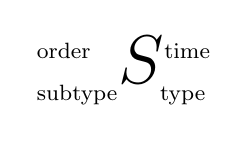
\begin{tikzpicture}[thick]
\node (S) at (0,0) {\Huge ${}_{\text{\footnotesize{subtype}}}^{\text{\footnotesize{order}}}S_{\text{\footnotesize{type}}}^{\text{\footnotesize{time}}}$};
\end{tikzpicture}


\end{document}
